\begin{frame}{Video-Pipeline}
\begin{columns}[T,onlytextwidth]
\begin{column}{0.52\textwidth}
\begin{enumerate}
    \item Video laden und Frames verarbeiten.
    \item Optional deinterlacen.
    \item Gesichter pro Frame detektieren.
    \item Blur-Maske auf erkannte Gesichtsregionen anwenden.
    \item Ergebnis in \texttt{Videos/lab\_outputs/} schreiben.
\end{enumerate}
\end{column}
\begin{column}{0.44\textwidth}
\begin{mynote}[Praxis]
\scriptsize
Die technische Modellqualität wird erst in der Videoausgabe wirklich sichtbar: verpasste Boxen bleiben sichtbare Gesichter.
\end{mynote}
\end{column}
\end{columns}
\vspace{0.1em}
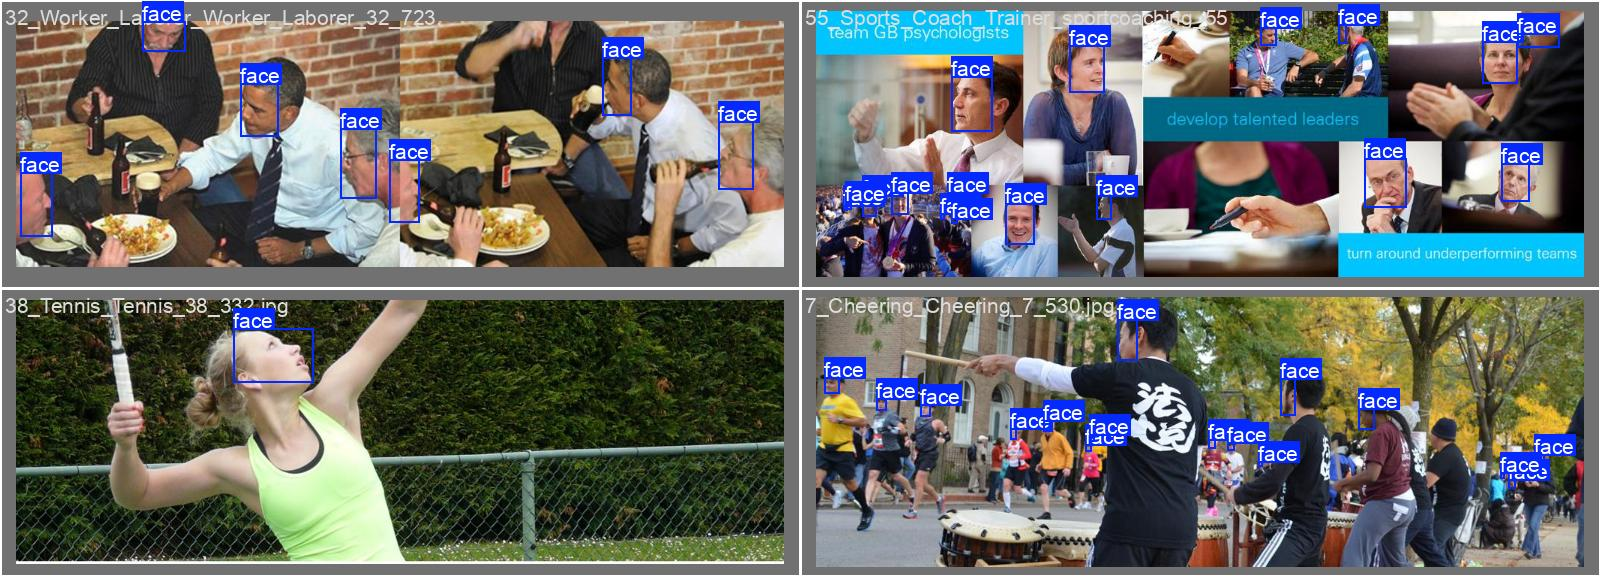
\includegraphics[width=\textwidth,height=0.18\textheight,keepaspectratio]{imglib/face_model_lab/yolo_val_labels.jpg}
\end{frame}
